\chapter{Metodologia}
\label{chap:metodologia}

\section{Visão Geral da Metodologia}

A Figura~\ref{fig:metodologia_fluxo} ilustra a sequência de fases que orientam a
pesquisa, desde a concepção teórica até a análise empírica dos resultados. Este
percurso metodológico assegura a rastreabilidade e a reprodutibilidade dos
procedimentos adotados para desenvolver e validar o sistema de geração de mapas
para jogos \textit{roguelike}.

\begin{figure}[!ht]
    \centering
    \Caption{\label{fig:metodologia_fluxo} Fluxograma das etapas metodológicas
        do trabalho.}
    \UFCfig{}{
        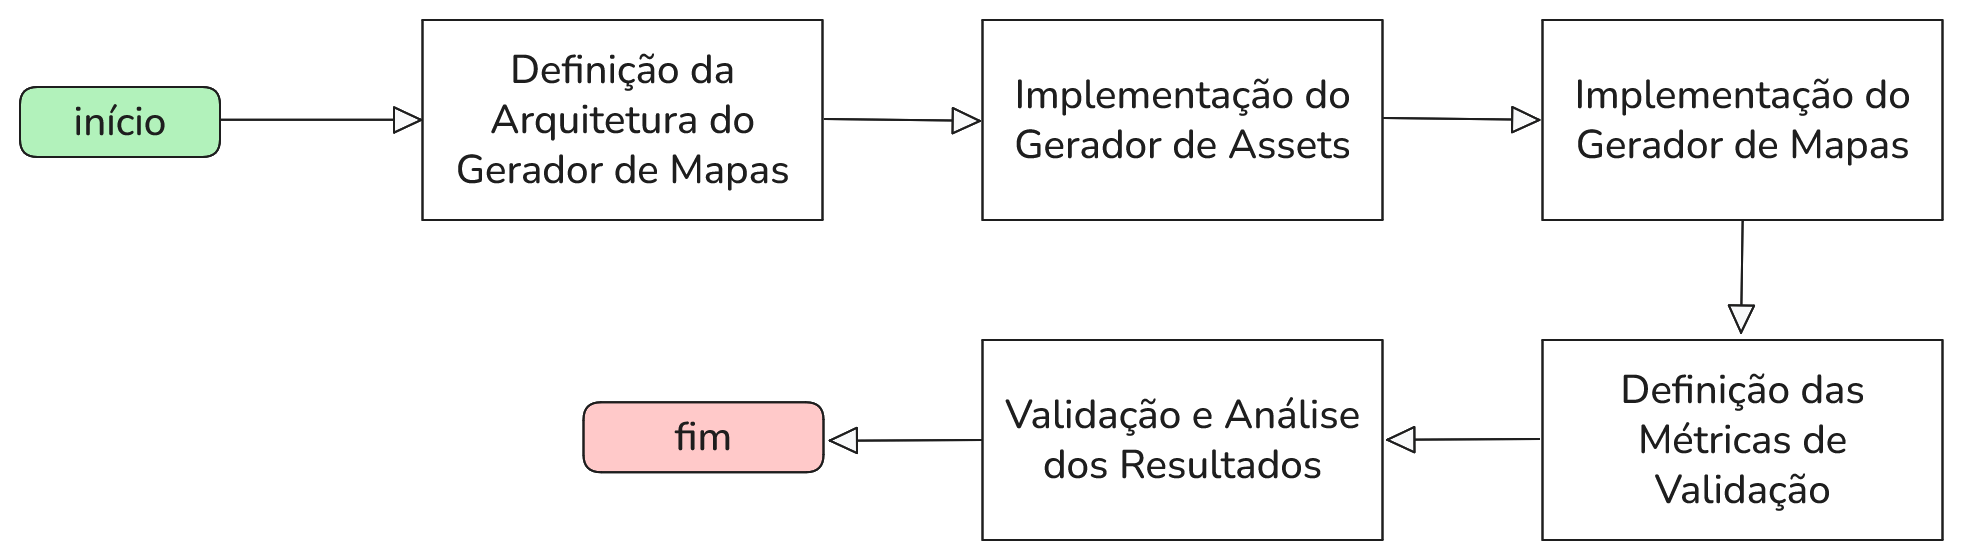
\includegraphics[width=0.9\textwidth]{figuras/metodology_two.png}
    }{
        \Fonte{Elaborado pelo autor}
    }
\end{figure}

%%%%%%%%%%%%%%%%%%%%%%%%%%%%%%%%%%%%%%%%%%%%%%%%%%%%%%%%%%%%%%%%%%%%%%%%%%%%%%%%
% Metodologia PARTE 1
%%%%%%%%%%%%%%%%%%%%%%%%%%%%%%%%%%%%%%%%%%%%%%%%%%%%%%%%%%%%%%%%%%%%%%%%%%%%%%%%

\section{Definição da Arquitetura do Gerador de Mapas}

A concepção da arquitetura deste sistema parte da identificação das limitações
intrínsecas aos \gls{LLM}s no que tange ao processamento de informações
geométricas e espaciais. Embora as \gls{LLM}s demonstrem capacidades
excepcionais na geração de texto e raciocínio semântico, o raciocínio espacial
permanece um desafio significativo.

Conforme demonstrado por \citeauthor{yan2023inherent},
modelos de estado da arte, como o \textit{GPT-4}, apresentam dificuldades
substanciais em tarefas que exigem compreensão precisa de coordenadas, como
plotar pontos em espaços 2D/3D ou executar algoritmos de busca de caminho. Esta
limitação é corroborada por \citeauthor{gallotta2024large}, que argumentam que,
apesar do potencial das \gls{LLM}s como assistentes de design, a falta de raciocínio
espacial impede que estes modelos gerem, de forma autônoma e consistente,
\textit{layouts} de níveis complexos que sejam jogáveis e estruturalmente coerentes,
requisitos fundamentais para o gênero \textit{roguelike}.

Durante a fase exploratória desta pesquisa, experimentos práticos corroboraram
essas dificuldades teóricas. Tentativas de utilizar o \gls{LLM} para gerar
diretamente a topologia e a disposição dos elementos resultaram em mapas
geometricamente inválidos. A Figura~\ref{fig:llm_topology_fail} ilustra um caso
específico onde o modelo falhou em manter a integridade da sala, resultando em
\textit{tiles} faltando no interior da estrutura e no "vazamento"\ de partes do
mapa para áreas desconexas. Tais erros evidenciam que a \gls{LLM}, quando
encarregada da estrutura espacial, tende a alucinar posições, comprometendo a
jogabilidade.

\begin{figure}[!ht]
    \centering
    \Caption{\label{fig:llm_topology_fail} Exemplo de falha na geração direta de
    topologia por LLM. Observam-se inconsistências estruturais graves,
    destacadas como \textit{tiles} ausentes no chão da sala e vazamento de
    estruturas para fora dos limites lógicos do mapa.}
    \UFCfig{}{
        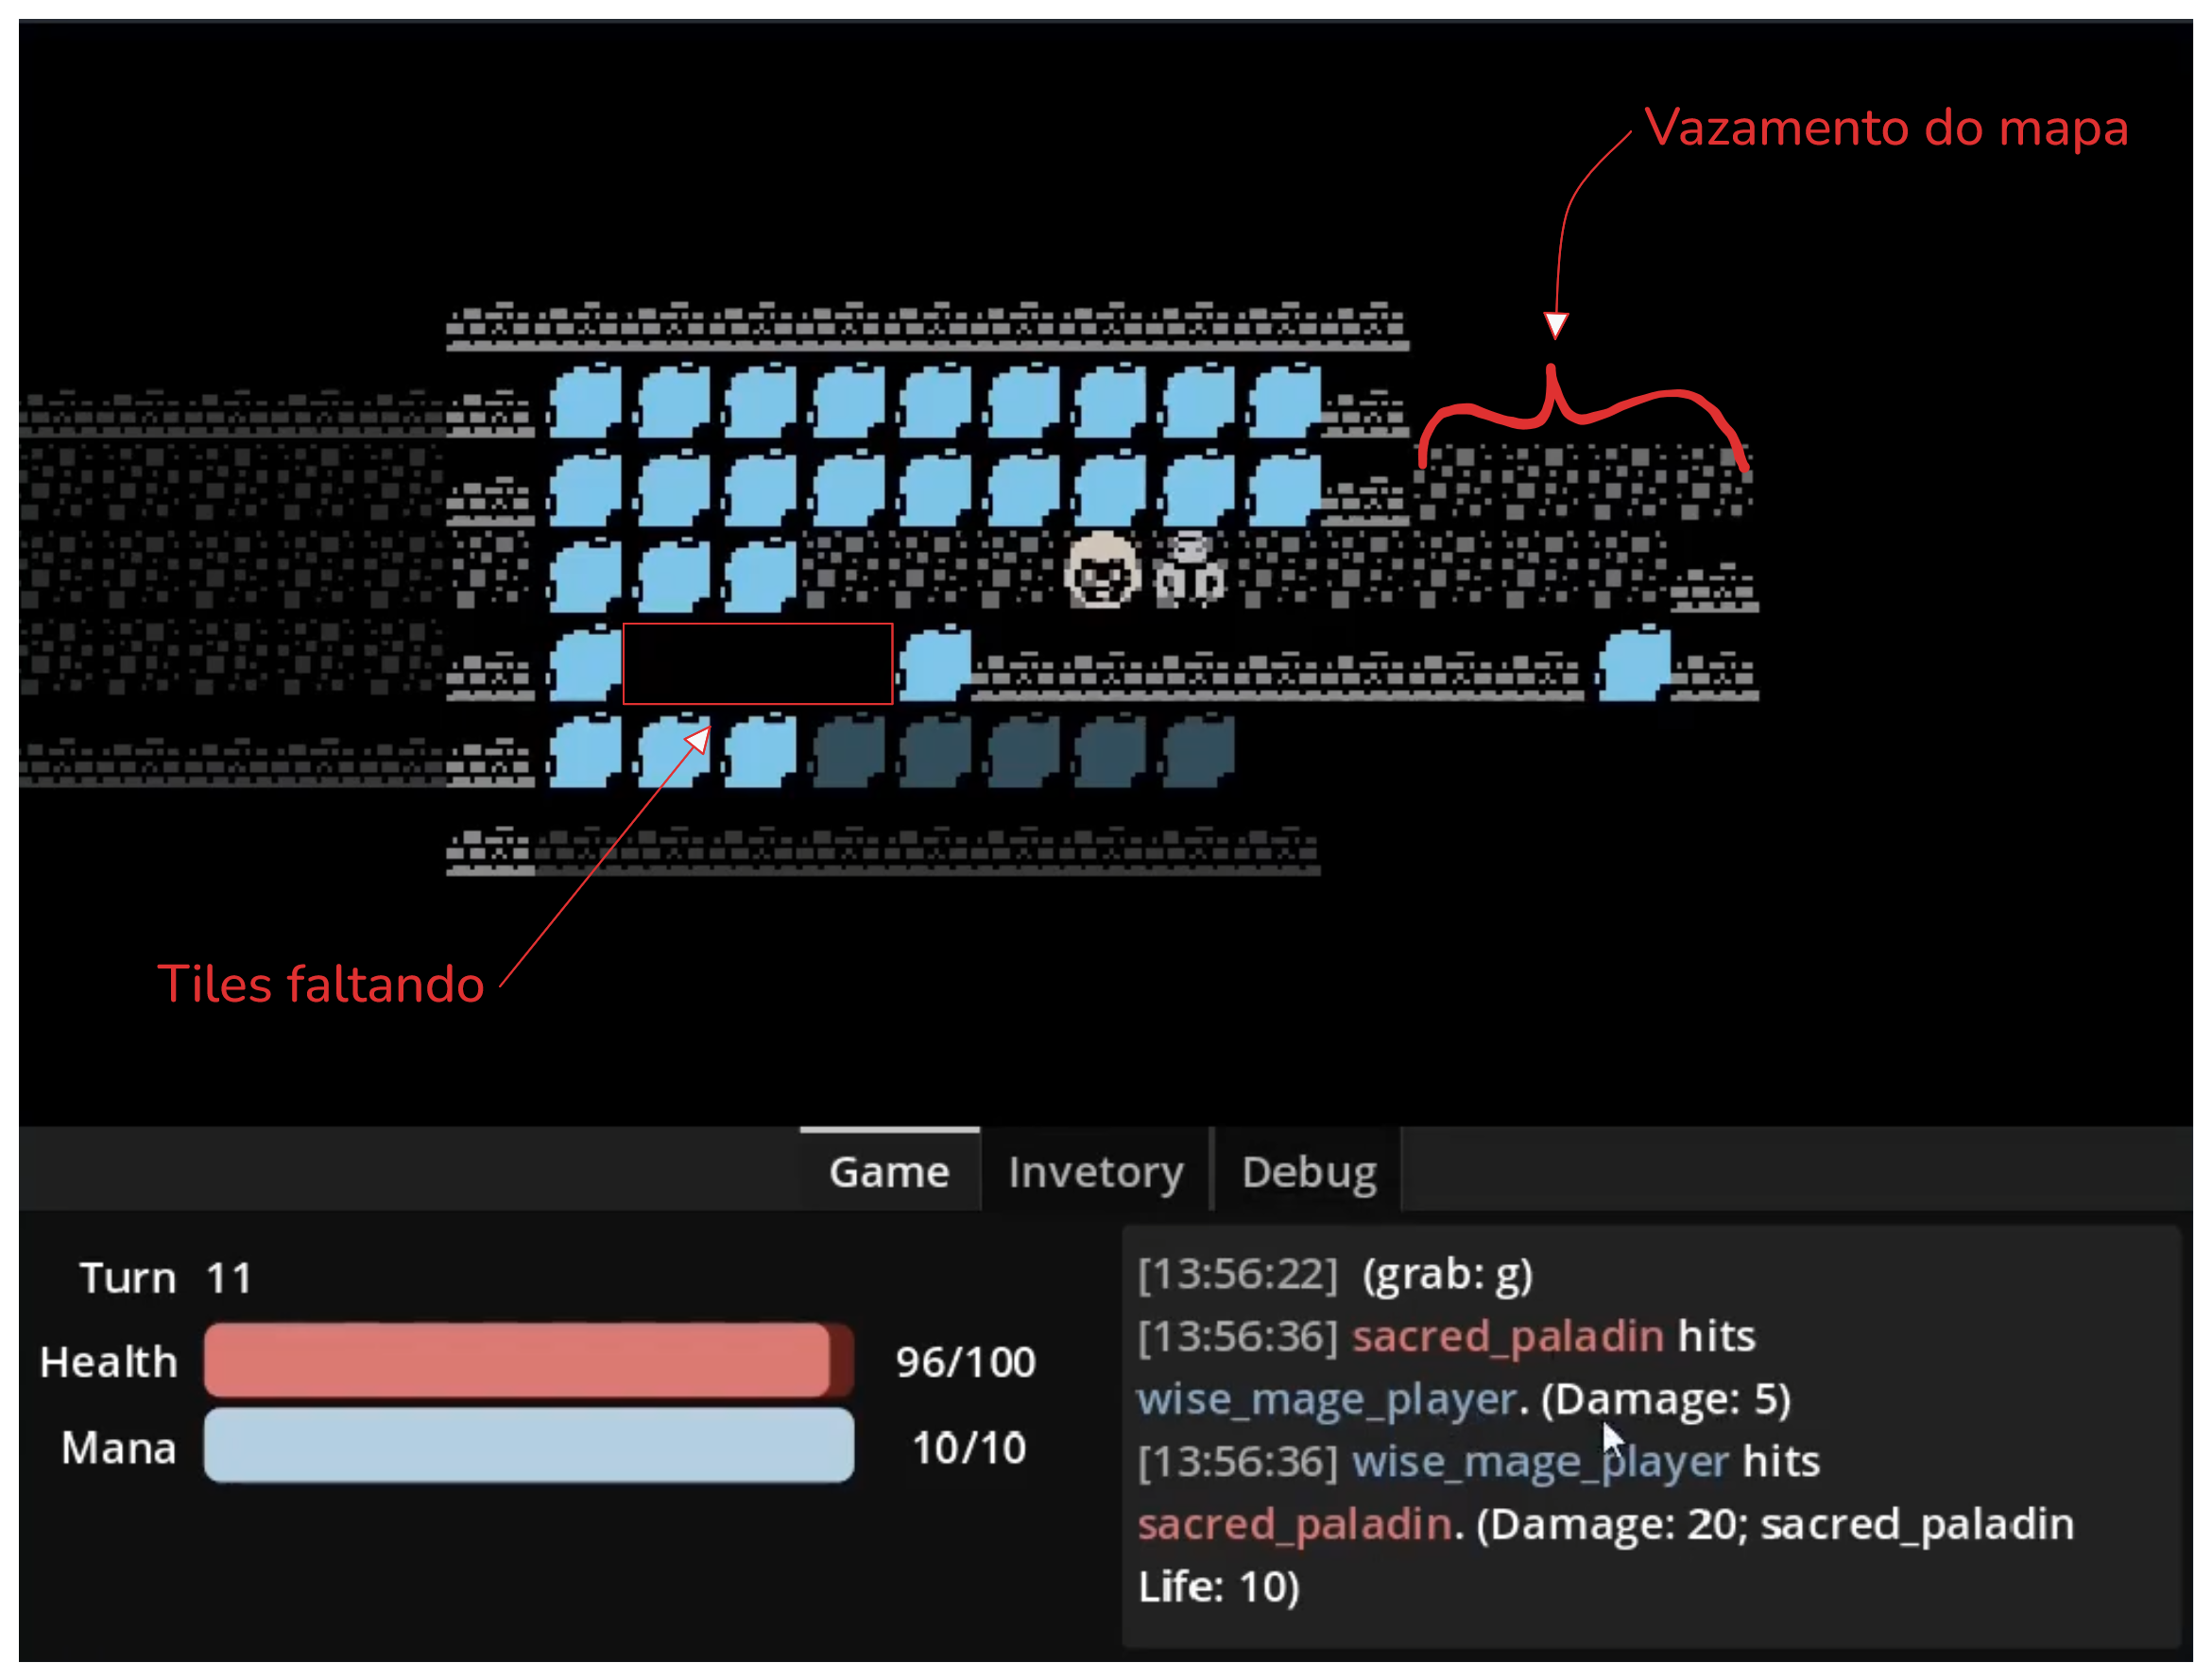
\includegraphics[width=0.9\textwidth]{figuras/generation_fail.png} 
    }{
        \Fonte{Elaborado pelo autor}
    }
\end{figure}

Diante deste cenário e das falhas observadas, este trabalho propõe uma
arquitetura híbrida que desacopla a responsabilidade criativa da
responsabilidade estrutural. A abordagem divide o processo de geração em dois
módulos distintos e complementares: o Gerador de \textit{Assets}, impulsionado
por \gls{LLM}, e o Gerador de Mapas, fundamentado em algoritmos de \gls{PCG}
tradicionais. A visão geral desta metodologia e o fluxo de dados entre os
componentes são apresentados na Figura~\ref{fig:geral_map_generation_flux}.

\begin{figure}[!ht]
    \centering
    \Caption{\label{fig:geral_map_generation_flux} Arquitetura Híbrida proposta:
        O fluxo inicia com a descrição do tema, que alimenta tanto o algoritmo de
        PCG quanto a \gls{LLM}. A \gls{LLM} gera assets semânticos (inimigos, itens e tiles)
        utilizando um Vector Store de texturas (RAG), enquanto o algoritmo de PCG
        utiliza esses assets para construir a estrutura espacial da masmorra.}
    \UFCfig{}{
        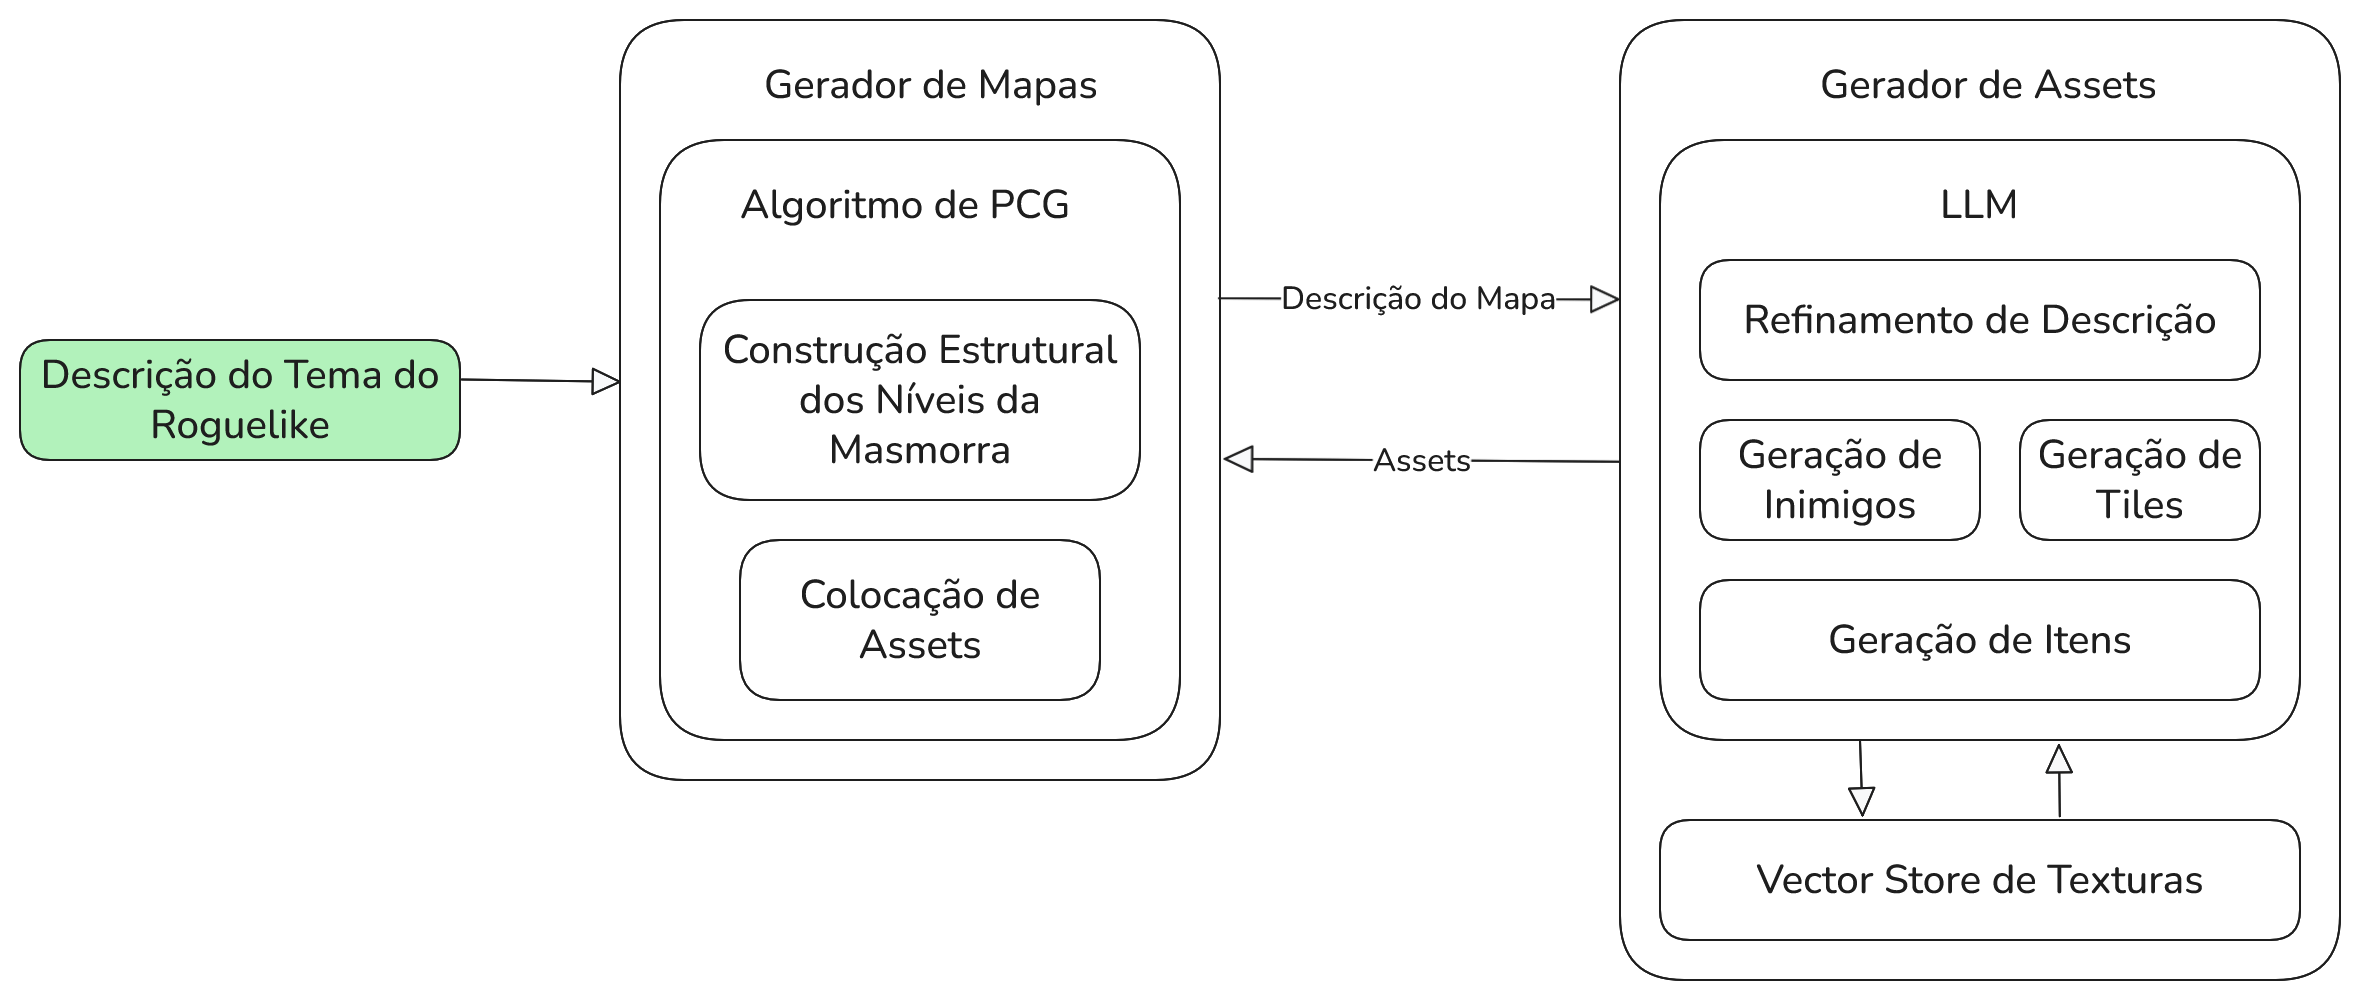
\includegraphics[width=0.8\textwidth]{figuras/geral_map_generetor_flux.png}
    }{
        \Fonte{Elaborado pelo autor}
    }
\end{figure}

\subsection{Geração de Assets via LLM}
Nesta etapa, a \gls{LLM} é utilizada para tarefas nas quais sua proficiência
semântica e criativa é maximizada. O modelo recebe como entrada o tema do
\textit{roguelike} e é responsável por gerar descrições detalhadas e instanciar
os \textit{assets} do jogo. Neste contexto, definem-se \textit{assets} como as
entidades que povoam o mapa: inimigos e itens consumíveis ou equipáveis.
A \gls{LLM}, portanto, enriquece o ambiente com contexto narrativo e visual, sem a
necessidade de gerenciar a topologia global da masmorra.

\subsection{Construção Estrutural via PCG Tradicional}
A segunda etapa assume a responsabilidade pela disposição espacial dos elementos
gerados anteriormente. Algoritmos clássicos de PCG, baseados em geração de
números pseudoaleatórios, são empregados para definir a geometria das salas, a
conectividade dos corredores e o posicionamento lógico dos \textit{assets}. O
algoritmo recebe a lista de objetos criados pela \gls{LLM} e os distribui pelo mapa
garantindo a validade topológica e a navegabilidade, contornando as limitações
espaciais das \gls{LLM}s apontadas por \citeauthor{yan2023inherent}.

Esta abordagem híbrida oferece duas vantagens principais. Primeiramente, a
\textbf{eficiência computacional}: delegar a estrutura do mapa para algoritmos
determinísticos ou estocásticos clássicos é significativamente menos custoso do
que realizar inferências complexas em uma \gls{LLM} para cada célula de uma
grade. Em segundo lugar, a arquitetura maximiza a \textbf{rejogabilidade}. Uma
única execução do Gerador de \textit{Assets} pode produzir um conjunto rico de
entidades temáticas que, por sua vez, podem ser recombinadas pelo algoritmo de
PCG para gerar uma quantidade virtualmente infinita de variações de mapas
distintos, preservando a essência de exploração e imprevisibilidade
característica dos jogos \textit{roguelike}.

%%%%%%%%%%%%%%%%%%%%%%%%%%%%%%%%%%%%%%%%%%%%%%%%%%%%%%%%%%%%%%%%%%%%%%%%%%%%%%%%
% Metodologia PARTE 2
%%%%%%%%%%%%%%%%%%%%%%%%%%%%%%%%%%%%%%%%%%%%%%%%%%%%%%%%%%%%%%%%%%%%%%%%%%%%%%%%

\section{Implementação do Gerador de Assets}
\label{sec:implementacao_assets}

A materialização de um jogo \textit{roguelike} requer não apenas a definição de
regras estruturais, mas também a criação de elementos tangíveis que povoam o
mundo virtual. Para garantir que inimigos, itens e ambientes compartilhem uma
identidade visual e narrativa coesa, o sistema não gera ativos isoladamente, mas
sim um objeto completo denominado \textit{Asset Bundle}.

O \textit{pipeline} de geração opera através de uma cadeia de requisições
sequenciais, desenhada para isolar o contexto e maximizar a precisão do \gls{LLM} em
cada tarefa específica. Conforme ilustrado na Figura~\ref{fig:pipeline_bundle}, o
fluxo de execução para a criação de um \textit{bundle} completo consiste em oito
etapas principais:

\begin{enumerate}
    \item \textbf{Descrição:} Entrada inicial do usuário (tema ou ideia).
    \item \textbf{Refinamento da Descrição:} Enriquecimento da descrição inicial do
          usuário para garantir maior detalhamento semântico.
    \item \textbf{Nomeação do Pacote de Assets:} Geração de um título temático para o pacote de ativos.
    \item \textbf{Definição do Jogador:} Criação da classe, história de fundo e aparência
          do avatar.
    \item \textbf{Geração do Objetivo Final:} Definição do artefato de vitória e sua
          justificativa narrativa.
    \item \textbf{Geração de Níveis:} Criação estruturada dos biomas e conjuntos de \textit{tiles}
          para cada profundidade da masmorra.
    \item \textbf{Geração de Armas:} Instanciação dos itens ofensivos com
          atributos de raridade e peso.
    \item \textbf{Geração de Inimigos:} Criação das entidades hostis com
          atributos de ameaça e peso.
    \item \textbf{RAG das Texturas:} Recuperação da textura em \textit{pixel
              art} mais semanticamente compatível no banco vetorial para cada entidade
          gerada nos passos anteriores.
\end{enumerate}

\begin{figure}[!ht]
    \centering
    \Caption{\label{fig:pipeline_bundle} Fluxo de geração do Pacote de Assets:
        da descrição inicial à instanciação dos objetos via RAG.}
    \UFCfig{}{
        % Substitua pelo nome correto do arquivo da imagem enviada
        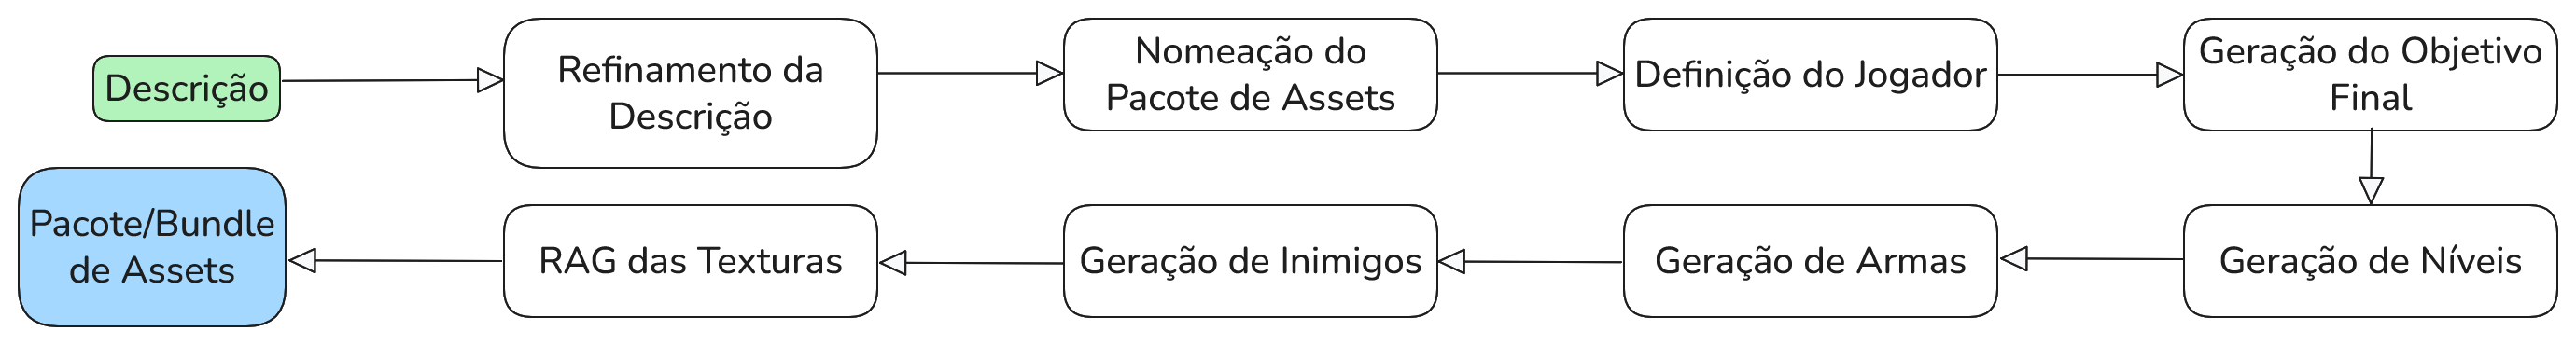
\includegraphics[width=\textwidth]{figuras/pipeline_geracao_bundle.png}
    }{
        \Fonte{Elaborado pelo autor}
    }
\end{figure}

O resultado final deste processo é um objeto \gls{JSON} estruturado que contém
todas as definições necessárias para que o Gerador de Mapas (descrito na Seção
\ref{sec:implementacao_mapas}) construa os níveis, popule as salas com inimigos
balanceados e distribua os itens de acordo com a progressão de dificuldade.

Para associar a capacidade gerativa dos \gls{LLM}s com representações visuais
concretas adotou-se a técnica de \gls{RAG}. Esta abordagem permite recuperar
texturas específicas de um banco vetorial com base em similaridade semântica,
uma estratégia validada recentemente na literatura por
\citeauthor{nasir2024word2world}, que utilizam \gls{LLM}s para gerar mundos 2D
completos integrando geração procedural e recuperação de ativos.

\subsection{Dataset e Pré-processamento Visual}

A base visual do sistema foi construída a partir do \textit{"1-Bit
    Pack"}\footnote{\textit{Kenney 1-Bit Pack} (Acesso em: 23 jan. 2026): \url{https://kenney.nl/assets/1-bit-pack}}
disponibilizado pelo site \textit{Kenney} sob licença \textit{Creative Commons
    CC0}. A escolha deste conjunto deve-se à sua alta diversidade temática e
consistência estilística, ideal para a prototipagem rápida de jogos
\textit{roguelike}. O pacote original contém 1078 \textit{tiles} de $16 \times
    16$ pixels, abrangendo desde elementos de interface de usuário até vegetação e
arquitetura, conforme ilustrado na Figura~\ref{fig:tilemap_kenney}.

\begin{figure}[!ht]
    \centering
    \Caption{\label{fig:tilemap_kenney} Tilemap completo do pacote \textit{"1-Bit Pack"}
        do site \textit{Kenney}, contendo a totalidade dos ativos gráficos disponíveis antes da
        filtragem.}
    \UFCfig{}{
        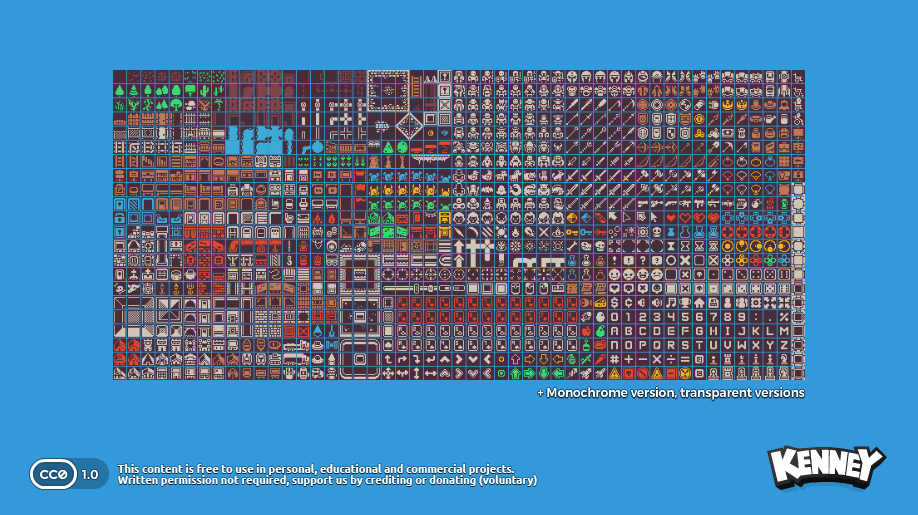
\includegraphics[width=0.8\textwidth]{figuras/kenney-1-bit-pack.png}
    }{
        \Fonte{Disponível em: https://kenney.nl/assets/1-bit-pack. Acesso em: 23 jan. 2026.}
    }
\end{figure}

Para garantir a precisão da busca vetorial e evitar a recuperação de elementos
inadequados, foi realizado um processo de curadoria e anotação manual. O
\textit{dataset} foi filtrado e segmentado em três categorias macro, totalizando
489 descrições textuais associadas a seus respectivos arquivos de imagem em
base64:

\begin{itemize}
    \item \textbf{Entities} (88 descrições): Inclui inimigos, \gls{NPC}s e o
          avatar do jogador.
    \item \textbf{Items} (183 descrições): Abrange poções, armas, armaduras,
          chaves e tesouros.
    \item \textbf{Environments} (218 descrições): Contém paredes, pisos,
          obstáculos naturais e vegetação.
\end{itemize}

Esta segmentação é crucial para evitar alucinações de categoria durante a
recuperação. Por exemplo, ao solicitar "uma espada longa", o sistema deve
restringir a busca ao subconjunto de \textit{Items}, eliminando a possibilidade
de retornar uma textura de parede ou chão que pudesse ter uma descrição vetorial
semanticamente próxima em um espaço latente não supervisionado.

\subsection{Stack Tecnológico e Busca Vetorial}

A implementação foi realizada na linguagem \textit{Python}, escolhida devido ao seu vasto
ecossistema de bibliotecas voltadas para Inteligência Artificial. A orquestração
do fluxo de dados utiliza o \textit{framework LangChain}, que facilita a
construção de agentes adaptáveis e a integração com modelos de linguagem. Para a
persistência e recuperação dos \textit{embeddings} das descrições dos
\textit{assets}, utilizou-se o \textit{ChromaDB}, um banco de dados vetorial
\textit{open-source} otimizado para busca semântica.

O núcleo do mecanismo de recuperação reside na função
\texttt{query\_vector\_store}. Esta função aceita três parâmetros principais: a
consulta textual (\texttt{query}), o tipo de armazenamento
(\texttt{store\_type}) para filtragem de categoria, e a quantidade de documentos
a recuperar (\texttt{documents\_count}), fixada em $n=1$ para esta aplicação. O
ChromaDB foi configurado para utilizar a Distância Euclidiana ao Quadrado
(\textit{Squared L2}) como métrica de similaridade, retornando o ativo cuja
descrição vetorial apresenta a menor distância em relação ao vetor da consulta
gerada pela LLM. A Figura~\ref{fig:query_vector_store} demonstra o
funcionamento prático deste módulo.

\begin{figure}[!ht]
    \centering
    \Caption{\label{fig:query_vector_store} Exemplos de execução da função de
        busca vetorial para três categorias distintas: Items ("A great sword"),
        Entities ("A dwarf") e Environments ("A stone wall").}
    \UFCfig{}{
        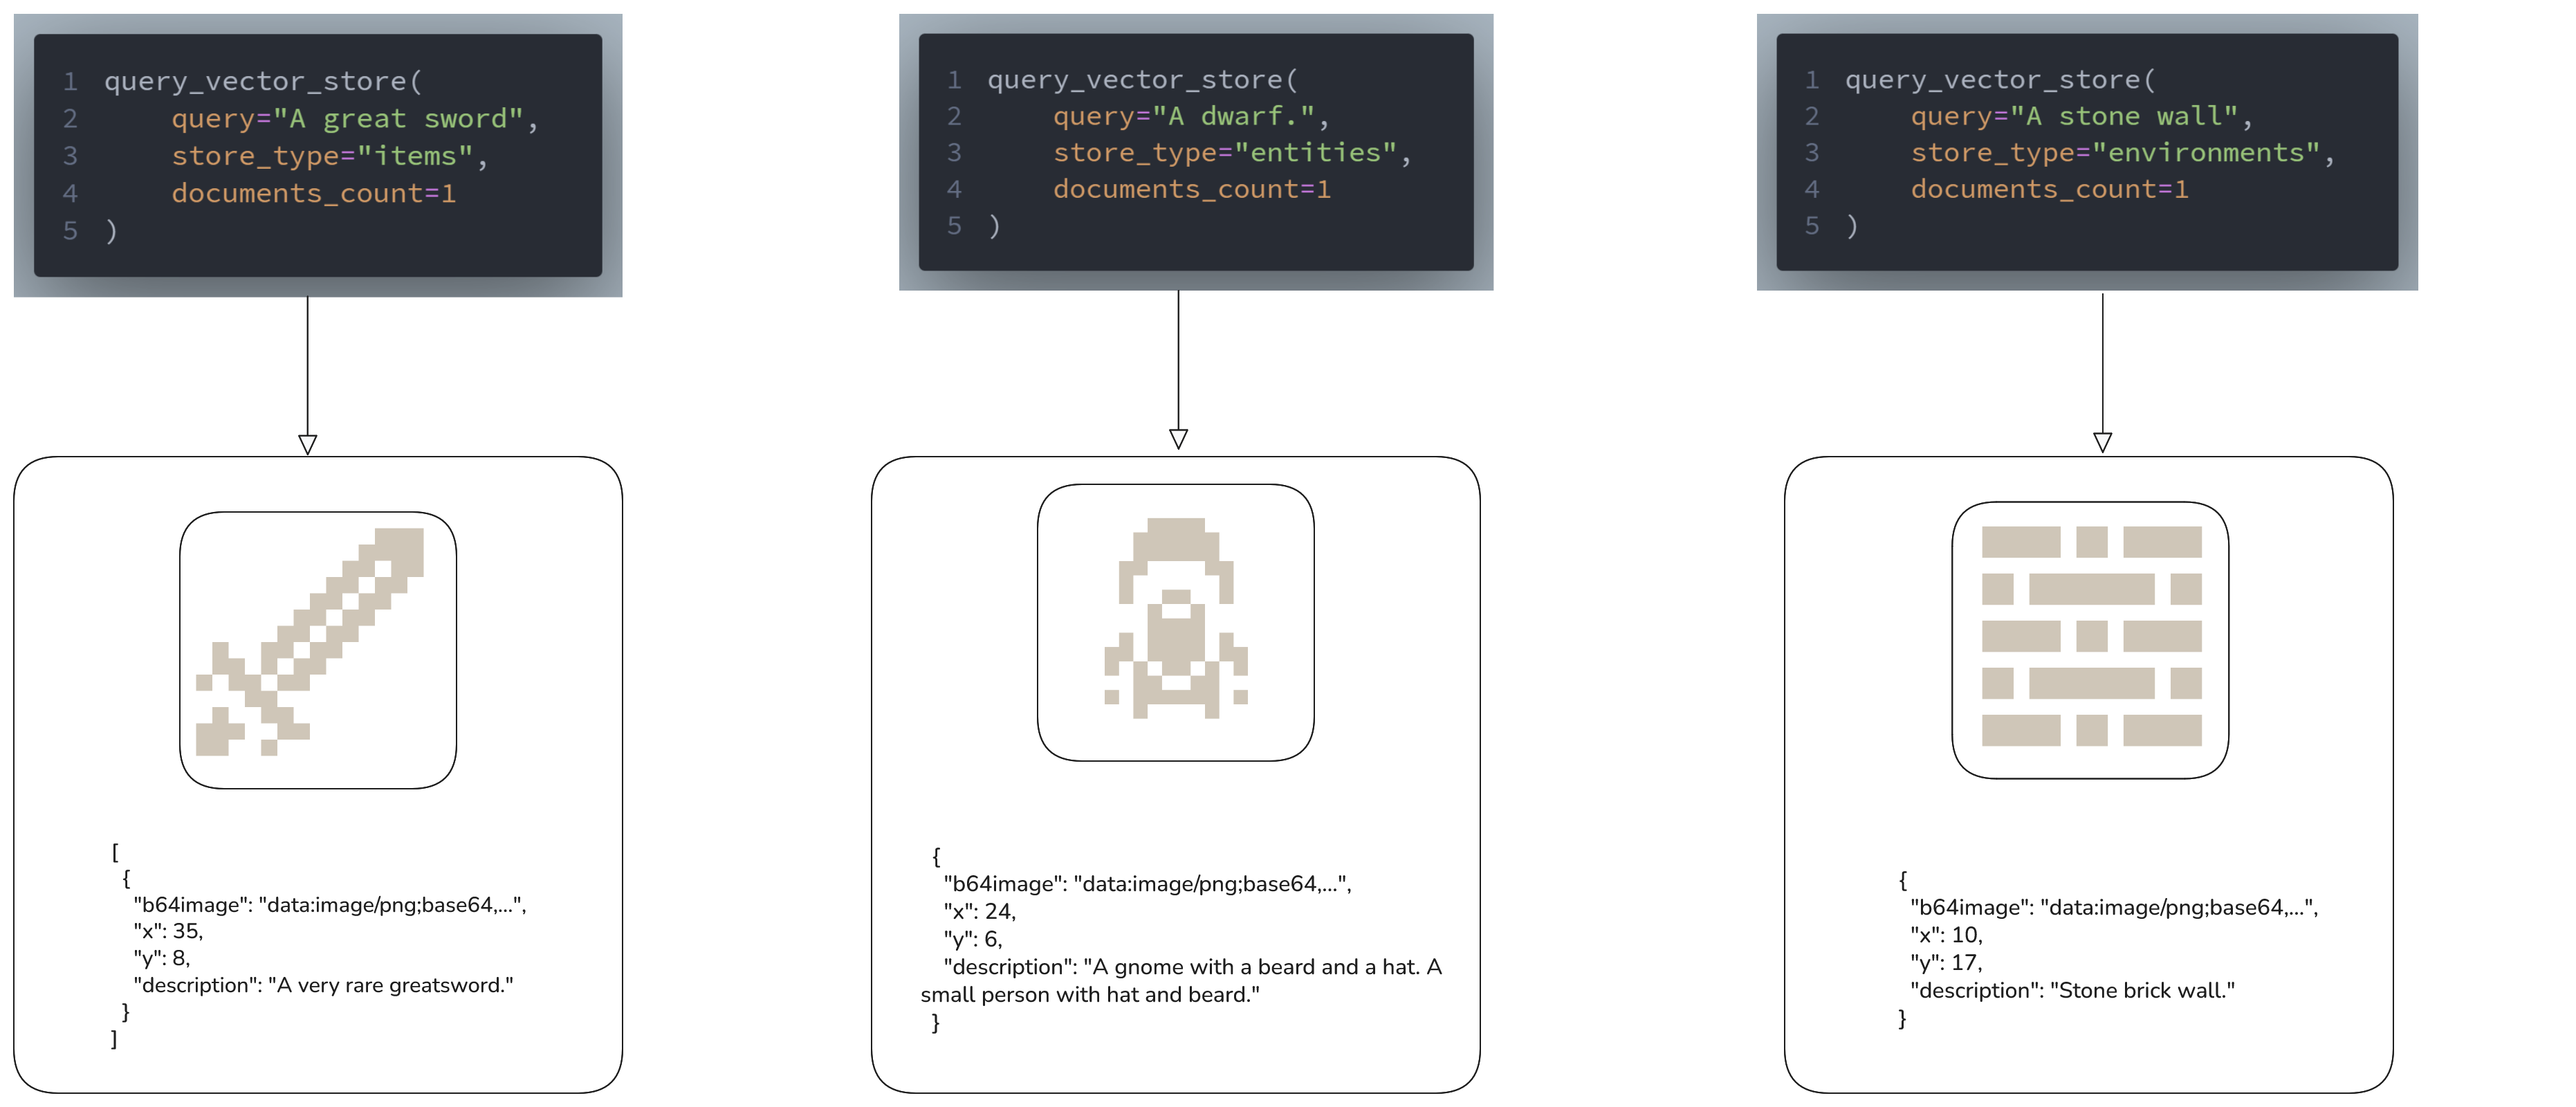
\includegraphics[width=0.8\textwidth]{figuras/query_vector_store.png}
    }{
        \Fonte{Elaborado pelo autor}
    }
\end{figure}

\subsection{Geração de Entidades com Saídas Estruturadas}

Um dos desafios recorrentes na utilização de \gls{LLM}s em sistemas de software é a
natureza não determinística e não estruturada das saídas textuais. Para mitigar
esse problema e garantir que o Gerador de Assets produza objetos de jogo
válidos, empregou-se o conceito de \textit{Structured Outputs}. Conforme
discutido por \citeauthor{shorten2024structuredrag}, a capacidade de forçar
modelos de linguagem a seguir esquemas rígidos, como \gls{JSON}, é essencial para o
desenvolvimento de sistemas de IA compostos.

Neste trabalho, a integração entre \textit{LangChain} e a biblioteca
\textit{Pydantic} foi utilizada para definir esquemas de dados rigorosos. Antes
de invocar a \gls{LLM}, define-se uma classe \textit{Pydantic} que representa o objeto de
jogo desejado (por exemplo, \texttt{MeleeWeapon}). A \gls{LLM} é então instruída
a preencher os campos desta classe com base na descrição temática fornecida pelo
usuário. O resultado é um objeto estruturado contendo não apenas os metadados do
item, mas também a
textura recuperada via \gls{RAG}.

\subsection{Abstração de Design e Valores Discretos}

Uma decisão de design fundamental na implementação foi a abstração dos atributos
numéricos dos objetos de jogo. Em vez de solicitar à \gls{LLM} que determine valores
brutos de dano ou pontos de vida (o que exigiria que o modelo mantivesse um
contexto complexo sobre o balanceamento matemático do jogo), optou-se pelo uso
de valores discretos em uma escala de 0 a 10 para atributos como \textit{rarity}
(raridade), \textit{threat} (ameaça) e \textit{weight} (peso).

Esta abordagem, ilustrada na Figura~\ref{fig:structured_flow}, desacopla a
geração criativa do balanceamento mecânico. A \gls{LLM} foca na coerência narrativa e
semântica (por exemplo, uma "Excalibur"\ deve ter raridade alta), enquanto o motor do
jogo traduz esses valores discretos em estatísticas finais (dano, vida,
armadura) através de multiplicadores definidos em arquivos de configuração.

\begin{figure}[!ht]
    \centering
    \Caption{\label{fig:structured_flow} Fluxo de geração de um asset
        estruturado: a descrição textual é processada, combinada com a textura
        recuperada do Vector Store e validada via Pydantic para criar um objeto de
        jogo funcional com atributos discretos.}
    \UFCfig{}{
        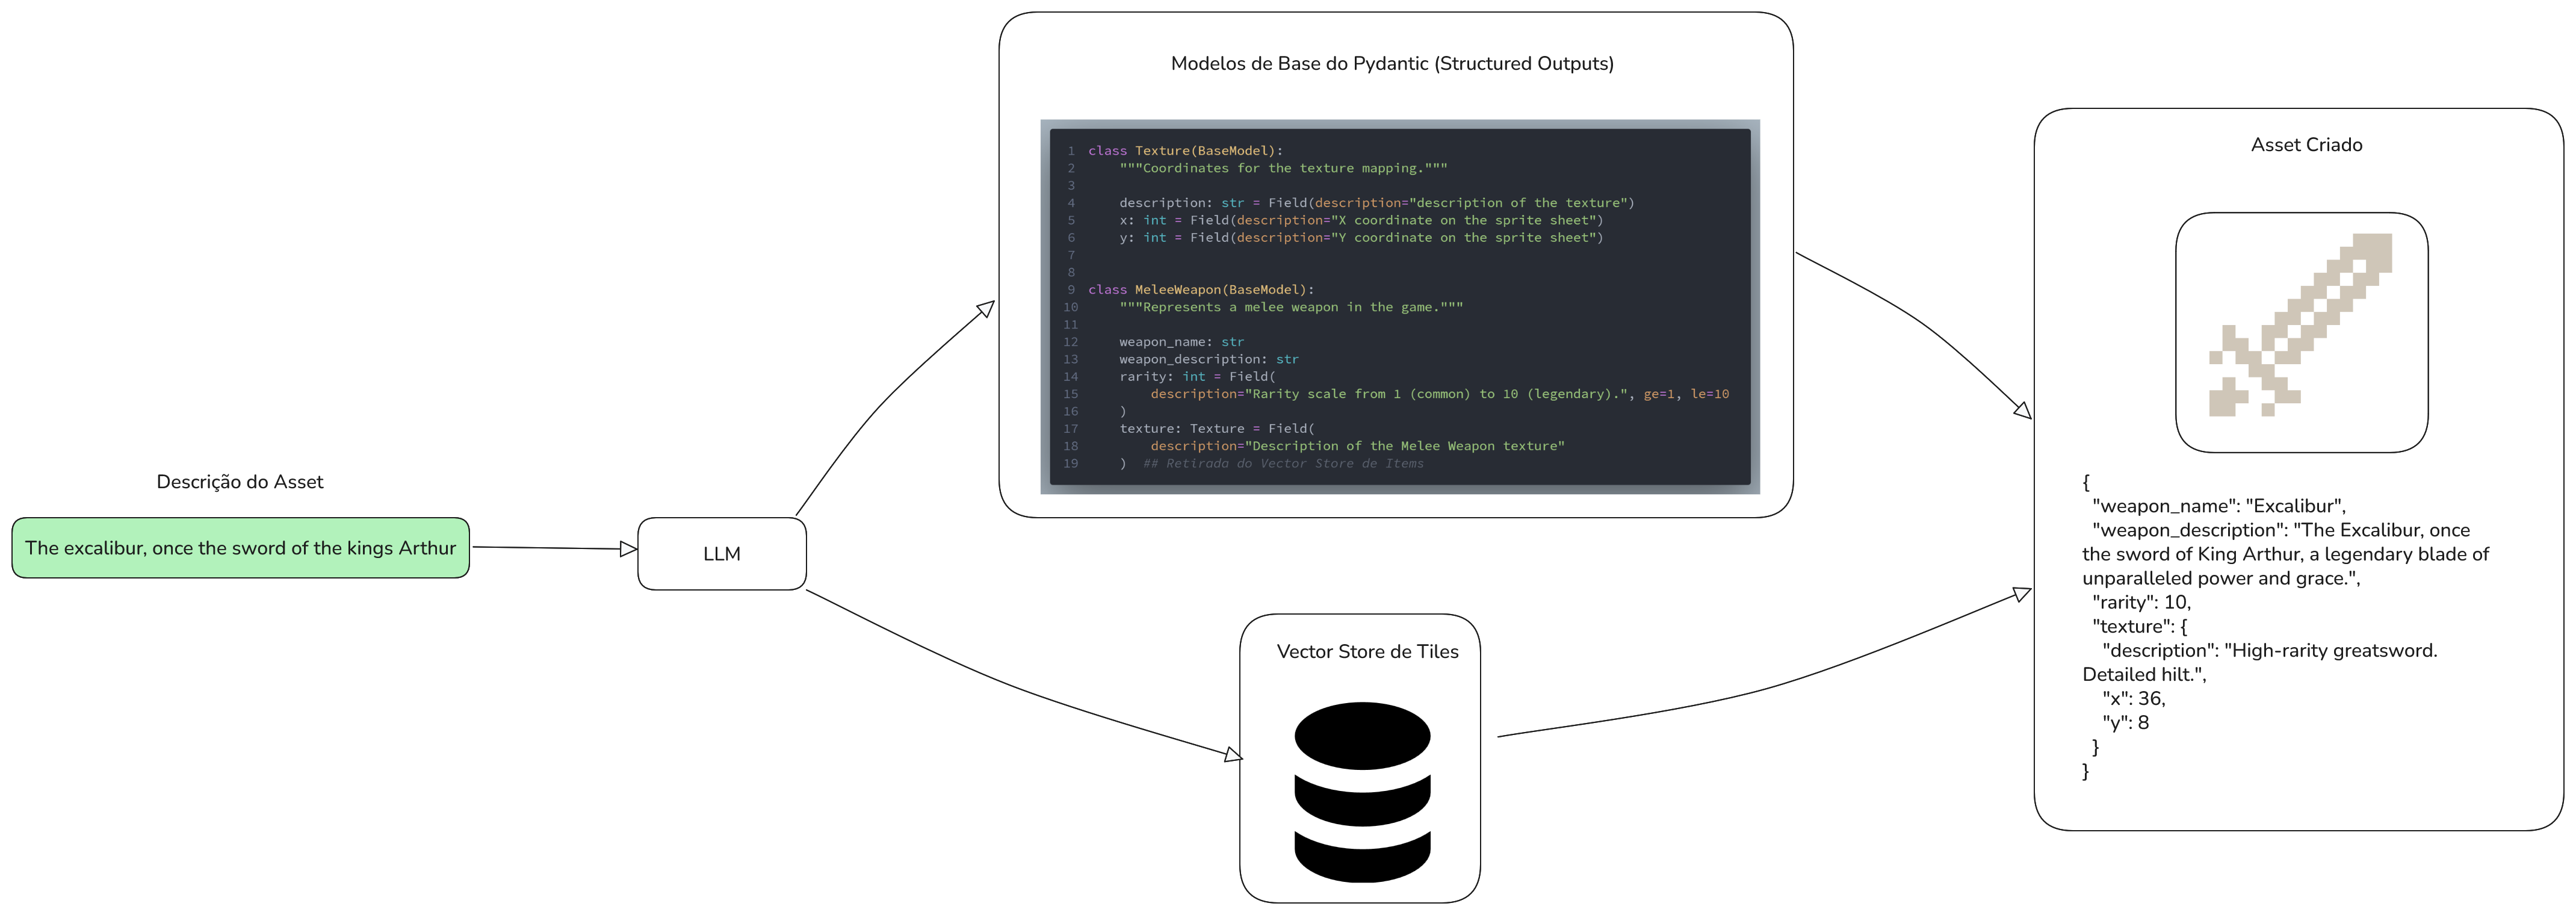
\includegraphics[width=\textwidth]{figuras/generating_asset.png}
    }{
        \Fonte{Elaborado pelo autor}
    }
\end{figure}

\subsection{Interface de Comunicação}

Para possibilitar a integração modular com o Gerador de Mapas e com a interface
do usuário, o Gerador de Assets foi encapsulado e exposto através de uma API
\gls{REST} desenvolvida com \textit{FastAPI}. A escolha desta arquitetura
justifica-se pela nativa compatibilidade com o formato \gls{JSON} gerado pelos
modelos \textit{Pydantic}, permitindo uma comunicação fluida e assíncrona entre
os componentes do sistema.

%%%%%%%%%%%%%%%%%%%%%%%%%%%%%%%%%%%%%%%%%%%%%%%%%%%%%%%%%%%%%%%%%%%%%%%%%%%%%%%%
% Metodologia PARTE 3
%%%%%%%%%%%%%%%%%%%%%%%%%%%%%%%%%%%%%%%%%%%%%%%%%%%%%%%%%%%%%%%%%%%%%%%%%%%%%%%%

\section{Implementação do Gerador de Mapas}
\label{sec:implementacao_mapas}

A segunda etapa da arquitetura híbrida proposta consiste no desenvolvimento do
Gerador de Mapas. Enquanto o módulo anterior é responsável pela criatividade
visual, este módulo assume a responsabilidade pela lógica espacial, validação
topológica e pela orquestração do ciclo de jogo.

\subsection{Escolha Tecnológica e Arquitetura Base}

Para a implementação do sistema, adotou-se a \textit{game engine} \textit{Godot} em sua
versão 4.5.1. A escolha justifica-se pela natureza \textit{open-source} da
ferramenta, que favorece a reprodutibilidade acadêmica e a transparência na
implementação de algoritmos. Segundo \citeonline{salmela2022game}, o \textit{Godot}
oferece uma integração robusta entre sua linguagem de \textit{scripting} nativa
(\textit{GDScript}) e o sistema de nós, facilitando o desenvolvimento de arquiteturas
modulares.

A implementação baseou-se na adaptação do tutorial \textit{"Complete Roguelike
    Tutorial"}\footnote{\textit{"Complete Roguelike
        Tutorial"} (Acesso em: 23 jan. 2026): \url{https://www.roguebasin.com/index.php/Complete\_Roguelike\_Tutorial,\_using\_python\%2Blibtcod}},
originalmente desenvolvido para a biblioteca \textit{libtcod} em \textit{Python},
hospedado no wiki comunitária \textit{RogueBasin}. A lógica original de
gerenciamento de turnos e Campo de Visão (\gls{FOV}) foi
portada para a arquitetura de nós do \textit{Godot}, aproveitando recursos nativos como:

\begin{itemize}
    \item \textbf{\textit{RandomNumberGenerator:}} Para garantir a estocasticidade
          determinística através do controle de \textit{seeds}, essencial para a
          \gls{PCG}.
    \item \textbf{\textit{HTTPRequest:}} Utilizado para comunicar-se de forma assíncrona
          com a API do Gerador de Assets desenvolvido na Seção
          \ref{sec:implementacao_assets}, recebendo os objetos em formato \gls{JSON}.
\end{itemize}

\subsection{Integração de Dados e Desserialização}

O desafio central desta etapa foi converter as descrições textuais e parâmetros
discretos gerados pela \gls{LLM} em objetos de jogo funcionais. Para isso, foi
implementada uma classe base denominada \texttt{Serializable}. Todos os objetos
dinâmicos do jogo (inimigos e itens) herdam desta classe.

A classe expõe o método \texttt{load(data: Dictionary)}, que atua como um
intérprete. Ao receber o \gls{JSON} da etapa anterior, este método instancia o nó
correspondente, aplica a textura recuperada via \gls{RAG} e atribui os valores de
atributos (como vida, dano e defesa) baseados nos valores discretos de
\textit{threat}, \textit{rarity} e \textit{weight} definidos pela \gls{LLM}.

\subsection{Algoritmo de Geração Estrutural}

Para a construção da topologia da masmorra, optou-se por um algoritmo de
Alocação de Retângulos Aleatórios com verificação de sobreposição. Esta técnica
garante salas estruturadas e conectadas, fundamentais para a navegação tática em
jogos \textit{roguelike}.

O algoritmo opera iterativamente tentando alocar salas dentro de um espaço
delimitado. Se uma nova sala não interceptar nenhuma das existentes, ela é
"esculpida"\ no mapa. A conectividade é garantida ligando-se o centro da nova
sala ao centro da sala anteriormente criada através de corredores em formato de
"L". O Algoritmo~\ref{alg:dungeon_gen_high_level} apresenta o pseudocódigo da
lógica implementada no método \texttt{generate\_basic\_dungeon}.

\begin{algorithm}[H]
    \caption{Geração Procedural da Estrutura da Masmorra}
    \label{alg:dungeon_gen_high_level}
    \SetAlgoLined

    % Definições locais para garantir funcionamento (se já estiver no preâmbulo, pode remover)
    \SetKwInput{Entrada}{Entrada}
    \SetKwInput{Saida}{Saída}
    \SetKwBlock{Inicio}{Início}{fim}
    \SetKwFor{Para}{para}{faça}{fim}
    \SetKwIF{Se}{SenaoSe}{Senao}{se}{então}{senão se}{senão}{fim}
    \SetKw{Retorna}{retorna}
    \SetKw{Continuar}{continuar}
    % -----------------------------------------------------------

    \Entrada{Restrições Geométricas ($D_{mapa}$), Limite de Tentativas ($N_{max}$)}
    \Saida{Topologia da Masmorra ($Salas$)}

    \Inicio{
        $Salas \leftarrow \emptyset$\;

        \Para{$i \leftarrow 0$ \textbf{até} $N_{max}$}{
            $Candidata \leftarrow$ GerarRetanguloAleatorio($D_{mapa}$)\;

            \Se{HaIntersecao($Candidata$, $Salas$)}{
                \Continuar\;
            }

            EscavarNoMapa($Candidata$)\;

            \Se{$Salas$ não está vazia}{
                $Alvo \leftarrow$ ObterUltimaSala($Salas$)\;
                CriarCorredorConectando($Alvo$, $Candidata$)\;
            }

            Adicionar $Candidata$ ao conjunto $Salas$\;
        }

        \Retorna $Salas$\;
    }
\end{algorithm}

\subsection{Povoamento e Progressão de Dificuldade}

Após a definição estrutural, o algoritmo popula as salas geradas. A distribuição
de entidades segue uma curva de progressão baseada na profundidade da masmorra.

O sistema utiliza os metadados gerados pela LLM na Seção
\ref{sec:implementacao_assets}. Itens e inimigos possuem atributos de
\textit{rarity}, \textit{threat}, \textit{weight}. O algoritmo de povoamento
calcula um peso probabilístico onde, quanto maior a profundidade do nível, maior
a chance de instanciar objetos com valores altos nesses atributos. Escadas são
posicionadas na última sala gerada, garantindo que o jogador precise atravessar
a estrutura para avançar.

\subsection{Ciclo de Gameplay e Condição de Vitória}

Para validar a integridade do gerador e a coerência dos assets criados, foi
implementado um ciclo de jogo completo. O design deste ciclo é inspirado
diretamente na estrutura de objetivos do jogo seminal \textit{Rogue}, conforme
detalhado em seu manual oficial \cite{epyx1985rogue}, onde o jogador deve
recuperar o Amuleto de \textit{Yendor} e retornar à superfície.  Nesta
implementação, o objetivo definido é descer através de níveis gerados
proceduralmente até encontrar o Artefato Final. Este artefato é um item
especial, também gerado pela \gls{LLM}, porém forçado a ter parâmetros de
raridade máxima e uma descrição narrativa de importância crítica.

A condição de vitória exige que o jogador colete o artefato e retorne vivo ao
primeiro nível da masmorra, invertendo o fluxo de progressão. Em conformidade
com as definições teóricas do gênero \textit{roguelike} apresentadas na
Seção~\ref{sec:roguelike-roguelites} e reforçadas pela estrutura clássica de
\textit{Rogue} \cite{epyx1985rogue}, o sistema implementa a mecânica de Morte
Permanente.  Caso os pontos de vida do jogador cheguem a zero em qualquer
momento da jornada, todo o progresso (incluindo o mapa explorado, itens
coletados e o próprio artefato) é perdido, e o jogo reinicia gerando uma nova
\textit{seed} aleatória, resultando em uma nova masmorra, mas utilizando os
mesmos assets gerados pela descrição textual.

%%%%%%%%%%%%%%%%%%%%%%%%%%%%%%%%%%%%%%%%%%%%%%%%%%%%%%%%%%%%%%%%%%%%%%%%%%%%%%%%
% Metodologia PARTE 4
%%%%%%%%%%%%%%%%%%%%%%%%%%%%%%%%%%%%%%%%%%%%%%%%%%%%%%%%%%%%%%%%%%%%%%%%%%%%%%%%

\section{Definição das Métricas de Validação}

A avaliação de conteúdo gerado proceduralmente, especialmente quando envolve
aspectos subjetivos como narrativa e estética, apresenta desafios inerentes que
dificultam o uso exclusivo de métricas quantitativas tradicionais. Para mitigar
essa questão e alinhar-se ao estado da arte na pesquisa de geração de mundos
virtuais, esta metodologia adota a abordagem de \textit{LLM-based Evaluation},
onde modelos de linguagem de larga escala atuam como juízes da qualidade do
conteúdo gerado. Esta estratégia é fundamentada nos trabalhos recentes de
\citeauthor{nasir2024word2world}, que utilizam \gls{LLM}s para pontuar a
coerência entre histórias e mundos 2D, e de
\citeauthor{huang2025word2minecraft}, que expandem o conceito para ambientes 3D,
aplicando análises de similaridade e reconstrução narrativa. Neste trabalho,
foram definidas duas métricas principais para validar a eficácia do
\textit{pipeline}: a \textbf{Coerência} e a \textbf{Reconstrução Semântica}.

\subsection{Métrica de Coerência (\textit{Coherence})}

Inspirada diretamente na metodologia proposta pelo sistema \textit{Word2World}
de \citeauthor{nasir2024word2world}, esta métrica visa quantificar o alinhamento
lógico e semântico entre a intenção textual e o artefato de jogo produzido. O
processo consiste em fornecer a uma \gls{LLM} avaliadora dois componentes
distintos:
\begin{enumerate}
    \item A descrição textual aprimorada e enriquecida (gerada na etapa anterior
          pela \gls{LLM});
    \item O conjunto de \textit{Assets} gerados em formato \gls{JSON} (resultado da
          aplicação de \gls{RAG} e \textit{Structured Outputs}).
\end{enumerate}

O modelo é instruído a atuar como um crítico e atribuir uma pontuação de 0 a
100, avaliando critérios como: a similaridade entre o ambiente descrito e os
elementos visuais selecionados; e a consistência dos inimigos e personagens.

É crucial destacar uma adaptação específica para o contexto deste trabalho: a
"descrição textual"\ fornecida para a avaliação não é a consulta inicial bruta do
usuário, mas sim a \textbf{descrição aprimorada} gerada pelo Gerador de
\textit{Assets}. Como o sistema converte a intenção do usuário em um contexto de
jogo \textit{Roguelike} (adicionando detalhes sobre masmorras, itens finais e
perigos específicos), a coerência deve ser medida em relação a este texto
refinado, garantindo que os objetos concretos do jogo reflitam as convenções do
gênero estabelecidas pelo próprio sistema.

\subsection{Métrica de Reconstrução Semântica}

Para complementar a avaliação direta, adota-se uma métrica de consistência
cíclica, similar à abordagem de \textit{reconstructed story-based similarity
    analysis} explorada por \citeauthor{huang2025word2minecraft}. Esta métrica testa
a capacidade dos ativos gerados de "comunicarem"\ seu tema de volta para um
observador, sem conhecimento prévio do \textit{prompt} original. O processo de
validação ocorre nas seguintes etapas:

\begin{enumerate}
    \item O conjunto de \textit{tiles} e ativos utilizados para compor o mapa
          (representados em \gls{JSON}) é submetido a uma \gls{LLM}.
    \item Solicita-se que o modelo descreva qual seria o tema, a ambientação e o
          possível enredo do jogo, baseando-se única e exclusivamente nos ativos
          fornecidos.
    \item A nova descrição gerada (texto reconstruído) é comparada com a
          \textbf{descrição aprimorada} original (utilizada na geração dos
          \textit{Assets}).
\end{enumerate}

A comparação quantitativa é realizada através da geração de \textit{embeddings}
para ambos os textos, utilizando a \textbf{Similaridade de Cosseno} para mensurar
a proximidade semântica no espaço vetorial. Uma similaridade maior (mais próxima
de 1) indica que o conjunto de ativos gerado preservou com sucesso as
características fundamentais do tema solicitado, a ponto de permitir que uma
inteligência artificial deduza a descrição original a partir apenas dos elementos
do jogo.